\chapter{Uczenie maszyn}
Uczenie maszynowe jest dziedzina algorytmów komputerowych, które automatycznie poprawiają swoją efektywność poprzez doświadczenie. 
Określa się je jako poddziedzinę sztucznej inteligencji. Algorytmy te pozwalają na zbudowanie matematycznego modelu na podstawie 
przykładowych danych nazywanych danymi treningowymi co pozwala im na wykonywanie predykcji lub decyzji bez potrzeby ich dokładnego 
zaimplementowania przez programistę. Uczenie maszynowe stosuje się do wielu zadań jak filtrowanie poczty mailowej ze spamu, reklamy Internetowe, 
wykrywanie twarzy na zdjęciach oraz nagraniach a przyszłości może pomóc w stworzeniu takich technologii jak 
samojezdne samochody. Sam termin został spopularyzowany przez informatyka Arhura Samuela w roku 1959, był on autorem pierwszego działającego 
systemu tego typu, jego program automatycznie grał w warcaby i uczył się na podstawie poprzednich potyczek.
\section{Rodzaje}
\begin{figure}[h!]
    \centering
    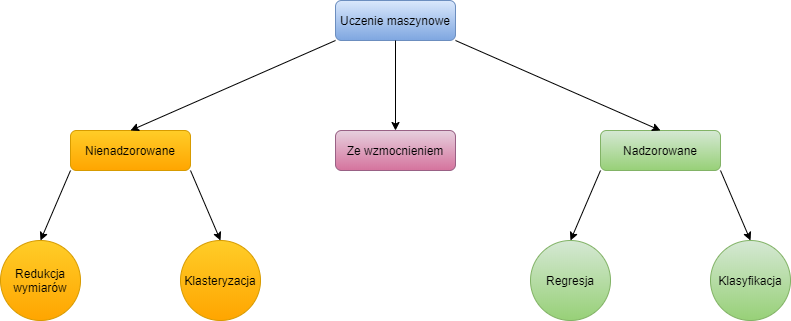
\includegraphics[width=1\textwidth]{./Img/typesofLearning.png}
    \caption{Rodzaje uczenia maszynowego Źródło: Własne}
\end{figure}
Algorytmy uczenia maszynowego można podzielić na trzy główne rodzaje w zależności od problemów, które mają one rozwiązywać są to:
\begin{enumerate}
    \item \textbf{Uczenie nadzorowane}
    Jest to najczęściej wykorzystywany rodzaj uczenia maszynowego polega on na tym 
    że maszyna uczy się na podstawie przykładów zawartych w danych treningowych 
    uczenie nadzorowane można porównać do nauczyciela i ucznia gdzie dane pełnią rolę nauczyciela 
    a program ucznia. Algorytmy tego typu potrafią znaleźć odpowiednie zależności na podstawie
    etykiet przypisanym danym,
    które następnie wykorzystują w celu predykcji wcześniej nie analizowanych danych.
    Ważnym zagadnieniem w przypadku uczenia nadzorowanego jest tak zwany Overfitting polegający 
    na przeuczeniu programu jednym zestawem treningowym przez co traci on umiejętność generalizacji problemu
    i nie jest w stanie poprawnie podejmować predykcji danych niewystarczająco podobnych
    do treningowych. Algorytmy tego typu można podzielić na dwa rodzaje:
    \begin{itemize}
        \item Klasyfikacja - przewidywanie kategorii
        \begin{itemize}
            \item rozpoznawanie elementów na zdjęciu
            \item filtrowanie spamu w skrzynce mailowej
        \end{itemize}
        \item Regresja - przewidywanie liczb
        \begin{itemize}
            \item przewidywanie trendów finansowych lub ekonomicznych
            \item prognozowanie pogody
        \end{itemize}
    \end{itemize}
    \item \textbf{Uczenie nienadzorowane}
    W przeciwieństwie do uczenia nadzorowanego uczenie nienadzorowane opiera się na braku
    nauczyciela a zadaniem maszyny jest znalezienie wzorców i zależności między analizowanymi
    obiektami samodzielnie. Wykorzystanie tego typu algorytmów pozwala na badanie danych nieoznaczonych,
    które są znacznie częsciej spotykane niż dane oznaczone. 
    \begin{itemize}
        \item Redukcja wymiarów
        \begin{itemize}
            \item Wizualizacja danych ``big data''
            \item Kompresja danych
        \end{itemize}
        \item Klasteryzacja
        \begin{itemize}
            \item Spersonalizowane reklamy
            \item Systemy rekomendacyjne
        \end{itemize}
    \end{itemize}
    \item \textbf{Uczenie ze wzmocnieniem}
    Uczenie ze wzmocnieniem polega na wykorzystaniu metody prób i błędów w taki sposób by maszyna została
    ``nagrodzona'' za wykonywanie czynności pożądanych oraz ``karana'' za popełnianie błędów. 
    Sukces takiego systemu oparty jest na odpowiedniej implementacji systemu nagród, który może 
    mieć całkowicie inne działanie w zależności od rozwiązywanego problemu. 
    Ponieważ algorytmy uczenia ze wzmocnieniem dążą do zebrania jak największej
    ilości ``nagrody'' nie zawsze odnajdują one optymalne rozwiązanie.
    \begin{itemize}
        \item Tworzenie programów grających w gry
        \item Samojezdne samochody
    \end{itemize}
\end{enumerate} 

\section{Algorytmy klasyfikacji}

\subsection{KNN}
\subsection{SVC}
\subsection{MLP}
\subsection{Binary trees}
\subsection{Naive Bayes}

\section{Wykorzystanie}

\section{Zagrożenia}
